Similar to the unconstrained case, we first prove the result for irreducible sources and then argue that the rate region of a general source is the same as that of an irreducible source that is obtained through reduction.
\begin{figure}[h]
\centering
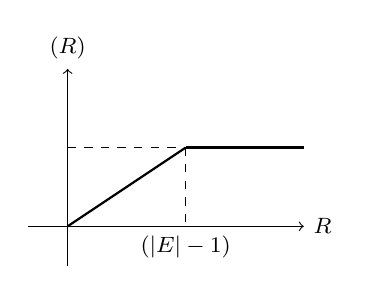
\begin{tikzpicture}
\tikzstyle{every node}=[font= \fontsize{8pt}{10pt}\selectfont]
    \draw [thin,  ->] (0,-0.5) -- (0,2)      % draw y-axis line
        node [above, black] {$\wskc(R)$};              % add label for y-axis
    
    \draw [thin,  ->] (-0.5,0) -- (3,0)      % draw x-axis line
        node [right, black] {$R$};              % add label for x-axis
    
    \draw [draw=black, thick] (0,0) -- (1.5,1);% draw the graph
    \draw [draw=black, thick] (1.5,1) -- (3,1);
    \draw [thin,  dashed] (0,1) -- (1.5,1);
    \draw [thin,  dashed] (1.5,1) -- (1.5,0);
    
    \node [left] at (0,1) {$\wskc$};                % label y-intercept
    \node [below] at (1.5,0) {$(|E|-1)\wskc$};               % label x-intercept
\end{tikzpicture}
\caption{$\wskc(R)$ curve denoting the wiretap secret key capacity at a given rate $R$ }
\label{fig:rateregion}
 \end{figure}
\begin{theorem}\label{thm:rate:irreducible}
Given an irreducible tree-PIN source $\RZ_V$ with a linear wiretapper $\RZ_w$, we have 
\begin{align*}
\wskc(R) = \min \left\{\frac{R}{|E|-1}, \wskc\right\} 
\end{align*}
where $R$ is the total discussion rate and $\wskc =\min_{e \in E}H(Y_e)$, which is the unconstrained wiretap secret key capacity.
\end{theorem}
\begin{proof}
Since the wiretapper side information can only reduce the secret key rate, $\wskc(R) \leq \skc(R)$. It follows from \cite[Theorem~4.2]{chan19} that $\skc(R) =  \min \left\{\frac{R}{|E|-1}, \skc\right\}$. Therefore, we have $\wskc(R) \leq \min \left\{\frac{R}{|E|-1}, \wskc\right\}$ because $\skc =\wskc$ for an irreducible tree-PIN source with a linear wiretapper, which was shown in Theorem~\ref{thm:cwsk:irred}.

For the achievability part, it is enough to show that the point $((|E|-1)\wskc,\wskc)$ is achievable because the rest of the curve follows from the time sharing argument between $((|E|-1)\wskc,\wskc)$ and $(0,0)$ ---  see Fig.~\ref{fig:rateregion}.

Let $s:=\wskc=\min_{e \in E}H(Y_e)=\min_{e \in E}n_e$, which is an integer. We will construct our achievable scheme on a sub-source  $\RZ'_V$ of the tree-PIN source $\RZ_V$ by ignoring some edge random variables. More precisely, $\RZ'_V$ is defined on the same tree $T$ with $\RY'_e := \left( \RX_{e,1}, \ldots, \RX_{e,s} \right)$ for each edge $e \in E$, and $\RZ'_i = \left( \RY'_e : i \in \xi (e) \right)$ for $i \in V$. Note that all the edge random vectors $\RY'_e$ have $s$ components. On the other hand, the  wiretapper side information $\RZ_{\opw}$ is the same as that of the original source. 

Let $\RX' :=(\RX_{e,k}: e\in E, 1 \leq k \leq s)$ and  $\RX'' :=(\RX_{e,k}: e\in E, s < k \leq n_e)$, which is a partition of the underlying components $\RX$ of the original source. This gives rise to a partition of the observations of the wiretapper into two parts: the first part contains observations involving only linear combinations of $\RX'$, and the second part contains linear observations with at least one component from $\RX''$. This means that $\RZ_{\opw}$, after applying some suitable invertible linear transformation, can be written as 
$$\RZ_{\opw} = \bM \RX' & \RX''\eM \bM \MA & \MB \\ \M{0} & \MC \eM ,$$ for some matrices $\MA$, $\MB$, and a full column-rank matrix $\MC$. With $\RZ'_{\opw}=\RX'\MA$ and $\RZ''_{\opw}=\RX'\MB + \RX''\MC$, $\RZ_{\opw} = \bM \RZ'_{\opw} & \RZ''_{\opw} \eM$.

For a large $n$,  users execute a linear secure omniscience communication scheme $\RF^{(n)}$ on the sub-source $\RZ'^n_V$ with respect to the wiretapper side information $\RZ^n_{\opw}$. Moreover, $\RF^{(n)}$ has the following properties: it achieves perfect omniscience at rate 
$$\frac{1}{n}H(\RF^{(n)})=H(\RZ'_V)-s=H(\RX')-s,$$ which is the minimum rate of omniscience $\rco(\RZ'_V)$, and it perfectly aligns with $\RZ'^n_{\opw}$, i.e., $H(\RZ'^n_{\opw}|\RF^{(n)})=0$. The existence of such a communication scheme is guaranteed from the proof of Theorem~\ref{thm:cwsk:irred}. After every user recovers the source $\RZ'^n_V$ using $\RF^{(n)}$, they agree on the key $\RK^{(n)}:=\RY'^n_{e_0}$ where $e_0 \in E$ is an edge incident on a leaf node. It is clear that $\RK^{(n)}$ satisfies the key recoverability condition because it is a function of the recovered source $\RZ'^n_V$. It remains to show that $\RK^{(n)}$ satisfies the secrecy condition.

Since $\RK^{(n)},\RZ'^n_{\opw}$ and $\RF^{(n)}$ are linear functions of $\RX'$, we have  $(\RK^{(n)}, \RF^{(n)}, \RZ'^n_{\opw}) - \RX'^n-\RZ''^n_{\opw}$. Note that $\RZ''^n_{\opw}$ is independent of $\RX'$ because $\MC$ is a full column-rank matrix. As a consequence, $\RZ''^n_{\opw}$ is independent of $(\RK^{(n)}, \RF^{(n)}, \RZ'^n_{\opw})$.  Furthermore, $\RY'^n_{e_0}$ is independent of $\RF^{(n)}$. This can be obtained by combining the perfect omniscience condition, which implies that $H(\RZ'^n_V|\RY'^n_{e_0},\RF^{(n)})=0$ for the leaf node, and the condition on the rate of the communication which is  $H(\RF^{(n)})=H(\RZ'^n_V)-ns=H(\RZ'^n_V)-H(\RY'^n_{e_0})$. Therefore, we have $H(\RY'^n_{e_0}|\RF^{(n)})= H(\RY'^n_{e_0},\RF^{(n)})-H(\RF^{(n)})=H(\RZ'^n_V,\RY'^n_{e_0},\RF^{(n)})-H(\RF^{(n)})=H(\RZ'^n_V)-H(\RF^{(n)})=H(\RY'^n_{e_0})$. The third equality is because $\RY'^n_{e_0}$ and $\RF^{(n)}$ are linear functions of $\RZ'^n_V$. Finally,
\begin{align*}
    H(\RK^{(n)}| \RF^{(n)}, \RZ^n_{\opw}) &=  H(\RK^{(n)}| \RF^{(n)}, \RZ'^n_{\opw},\RZ''^n_{\opw})\\
    &\utag{a}{=}  H(\RK^{(n)}| \RF^{(n)}, \RZ'^n_{\opw})\\
    &\utag{b}{=} H(\RK^{(n)}| \RF^{(n)})\\
    &= H(\RY'^n_{e_0}| \RF^{(n)})\\
    &\utag{c}{=}H(\RY'^n_{e_0})\\
    &= H(\RK^{(n)})
\end{align*}
where (a) follow from the independence of $\RZ''^n_{\opw}$ and $(\RK^{(n)}, \RF^{(n)}, \RZ'^n_{\opw})$, (b) is due that the fact that $\RF^{(n)}$ aligns perfectly with $\RZ'^n_{\opw}$, i.e., $H(\RZ'^n_{\opw}|\RF^{(n)})=0$ and (c) is because $\RY'^n_{e_0}$ is independent of $\RF^{(n)}$.

Thus we have shown that a secret key of rate $\frac{1}{n}H(\RK^{(n)})=\frac{1}{n}H(\RY'^n_{e_0})=s$ is achievable with a communication of rate $\frac{1}{n}H(\RF^{(n)})=H(\RZ'_V)-s= (|E|-1)s$. So the pair $((|E|-1)\wskc,\wskc)= ((|E|-1)s,s)$  is achievable, which is as desired.
\end{proof}

To extend this result to the general tree-PIN case, we will prove the following lemma, which allows us to carry out a reduction to an irreducible source without changing $\wskc(R)$. This lemma along with the above theorem on irreducible sources proves Theorem~\ref{thm:rateconstrained_treepin}. 

\begin{lemma}\label{lem:irred:rate} 
 If a tree-PIN source with a linear wiretapper $(\RZ_V,\RZ_{\opw})$ is not irreducible then there exists an irreducible source $(\tRZ_V, \tRZ_{\opw})$ such that 
 \begin{align*}
\wskc(\RZ_V\| \RZ_{\opw})(R) = \wskc(\tRZ_V\|\tRZ_{\opw})(R),\\ 
H(\RY_e|\op{mcf}(\RY_e\wedge\RZ_{\opw})) = H(\tRY_e)
\end{align*}
for all $e \in E$ and all discussion rates $R \geq 0$.
\end{lemma}
\begin{proof}
Since $(\RZ_V, \RZ_{\opw})$ is not irreducible, there exists an edge $e \in E$ such that $\RG_e := \op{mcf}(\RY_e\wedge \RZ_{\opw})$ is a non-constant function. Similar to the proof of Lemma~\ref{lem:irred:rate}, we linearly transform $\RY_e$ and $\RZ_{\opw}$ to  $(\RG_e, \tRY_e)$ and $(\RG_e, \tRZ_{\opw} )$, respectively where $ H(\tRY_e)=H(\RY_e|\op{mcf}(\RY_e\wedge\RZ_{\opw}))$. Let us consider a  new tree-PIN  source $\tRZ_V$, which is the same as $\RZ_V$ except that  $\tRY_e$ and $\tilde{n}_e$ are associated to the edge $e$, and the wiretapper side information is  $\tRZ_{\opw}$. Note that $(\tRZ_V, \tRZ_{\opw})$ is also a tree-PIN source with a linear wiretapper, and $\RG_e$ is independent of $(\tRZ_V, \tRZ_{\opw})$.

Since any valid scheme on reduced model $(\tRZ_V, \tRZ_{\opw})$ can be used as a valid scheme on original model $(\RZ_V, \RZ_{\opw})$, we have 
$$\wskc(\RZ_V\| \RZ_{\opw})(R) \geq \wskc(\tRZ_V\|\tRZ_{\opw})(R).$$

To prove the reverse inequality, $\wskc(R):=\wskc(\RZ_V\| \RZ_{\opw})(R) \leq \wskc(\tRZ_V\|\tRZ_{\opw})(R)$, consider capacity-optimal schemes. Fix $\delta>0$, and let $(\RF^{(n)},\RK^{(n)})$ be a WSKA scheme whose key rate and communication rate satisfy
\begin{gather}
    \wskc(R)-\delta < \liminf \frac{1}{n}\log|\mc{K}^{(n)}| < \wskc(R), \label{eq:rate_k}\\
    \limsup \frac{1}{n}\log|\mc{F}^{(n)}| < R. \nonumber
\end{gather}
Let $L:=\liminf \frac{1}{n}\log|\mc{K}^{(n)}|$. Fix an $\epsilon>0$ small enough that $(L-7\epsilon, L+7\epsilon) \subseteq (\wskc(R)-\delta, \wskc(R))$.
We restrict to a subsequence of $\left(\frac{1}{n}\log|\mc{K}^{(n)}|\right)_{n\geq 1}$ whose limit is $L$. And, with an abuse of notation, we still index this sequence\footnote{Designing a protocol on a subsequence can easily be extended to all the integers without sacrificing the asymptotic performance of the protocol.} with $n$. Therefore, for all $n$ large enough,  $L-\epsilon <\frac{1}{n}\log|\mc{K}^{(n)}| < L+\epsilon$. Again, along this subsequence, we have $\limsup \frac{1}{n}\log|\mc{F}^{(n)}| < R$ because of the properties of subsequential limits. Moreover, we have  $0 \leq \log|\mc{K}^{(n)}|-H(\RK^{(n)}|\RZ^n_{\opw},\RF^{(n)})=\left[\log|\mc{K}^{(n)}|-H(\RK^{(n)})\right] +I(\RK^{(n)} \wedge \RZ^n_{\opw},\RF^{(n)})< \epsilon$ and $\Pr\left[ \exists j\in V \text{ s.t. }  \RK_j^{(n)}\neq \RK^{(n)}\right]< \epsilon$ for all $n$ large enough.

Note that the above secrecy  condition implies that $0\leq\left[\log|\mc{K}^{(n)}|-H(\RK^{(n)})\right] < \epsilon$ and  $I(\RK^{(n)}\wedge\tRZ^n_{\opw},\RG^n_e,\RF^{(n)})=I(\RK^{(n)}\wedge\RZ^n_{\opw},\RF^{(n)})<  \epsilon$. The latter condition implies that $I(\RK^{(n)}\wedge\tRZ^n_{\opw},\RF^{(n)}|\RG^n_e)<  \epsilon$ and $I(\RK^{(n)}\wedge \RG^n_e)<  \epsilon$. From all the above conditions, we have
\begin{gather}
L-\epsilon <\frac{1}{n}\log|\mc{K}^{(n)}| < L+\epsilon,\label{eq:rate1}\\
    0\leq\left[\log|\mc{K}^{(n)}|-H(\RK^{(n)})\right] < \epsilon,\label{eq:rate2}\\
    I(\RK^{(n)}\wedge\tRZ^n_{\opw},\RF^{(n)}|\RG^n_e)<  \epsilon,\label{eq:rate3}\\ I(\RK^{(n)}\wedge \RG^n_e)<  \epsilon.\label{eq:rate4}
\end{gather}
Let $\mc{K}^{(n)}_g$ be the range of $\RK^{(n)}$ when $\RG_e^n=g$, and similarly, $\mc{F}^{(n)}_g$ denote the range of $\RF^{(n)}$ when $\RG_e^n=g$. Note that since $\mc{K}^{(n)}_g \subseteq \mc{K}^{(n)}$ and $\mc{F}^{(n)}_g \subseteq \mc{F}^{(n)}$ for any $g$, we have $\log|\mc{K}^{(n)}_g|\leq \log|\mc{K}^{(n)}|$ and $\log|\mc{F}^{(n)}_g|\leq \log|\mc{F}^{(n)}|$, hence
\begin{gather}
    \sum_{g}\Pr(\RG_e^n=g)\log|\mc{K}^{(n)}_g|\leq  \log|\mc{K}^{(n)}|.\label{eq:rate5}
\end{gather}
We will show that there exists a realization $g^{*}$ of $\RG_e^n$ for which all the desired conditions are met.

From \eqref{eq:rate2}, \eqref{eq:rate4} and \eqref{eq:rate5}, we obtain
\begin{gather*}
    H(\RK^{(n)}|\RG^n_e)\leq \sum_{g}\Pr(\RG_e^n=g) \log|\mc{K}^{(n)}_g|\leq \log|\mc{K}^{(n)}| < H(\RK^{(n)}|\RG^n_e)+2\epsilon.
\end{gather*}
We can conclude from the above chain of inequalities that 
\begin{gather*}
    0\leq \sum_{g}\Pr(\RG_e^n=g)\left[\frac{1}{n} \log|\mc{K}^{(n)}|-\frac{1}{n} \log|\mc{K}^{(n)}_g|\right]< 2\epsilon,\\
    0\leq \sum_{g}\Pr(\RG_e^n=g)\left[ \log|\mc{K}_g^{(n)}|-H(\RK^{(n)}|\RG^n_e=g)\right]< 2\epsilon.
\end{gather*}
These inequalities together with \eqref{eq:rate3} give
\begin{align*}
    0\leq &\sum_{g}\Pr(\RG_e^n=g)\left\lbrace\left[\frac{1}{n} \log|\mc{K}^{(n)}|-\frac{1}{n} \log|\mc{K}^{(n)}_g|\right]+\left[ \log|\mc{K}_g^{(n)}|-H(\RK^{(n)}|\RG^n_e=g)\right]\right. \\ &\left.+\, I(\RK^{(n)}\wedge\tRZ^n_{\opw},\RF^{(n)}|\RG^n_e=g)+\Pr\left( \exists j\in V \text{ s.t. } \RK_j^{(n)}\neq \RK^{(n)}\Bigm\vert \RG^n_e=g\right)\right\rbrace < 5\epsilon.
\end{align*}
Note that the averaged quantity (the term in the curly bracket) is non-negative; hence there exists a realization of $\RG_e^{(n)}=g^*$ such that 
\begin{align*}
    0\leq &\left[\frac{1}{n} \log|\mc{K}^{(n)}|-\frac{1}{n} \log|\mc{K}^{(n)}_{g^*}|\right]+\left[ \log|\mc{K}_{g^*}^{(n)}|-H(\RK^{(n)}|\RG^n_e={g^*})\right]\\ &+\,I(\RK^{(n)}\wedge\tRZ^n_{\opw},\RF^{(n)}|\RG^n_e={g^*})+\Pr\left( \exists j\in V \text{ s.t. } \RK_j^{(n)}\neq \RK^{(n)}\Bigm\vert \RG^n_e=g\right) < 5\epsilon.
\end{align*}
Since all the summands are non-negative, we have 
\begin{subequations}
\label{eq:rate6}
\begin{gather}
    0\leq \left[\frac{1}{n} \log|\mc{K}^{(n)}|-\frac{1}{n} \log|\mc{K}^{(n)}_{g^*}|\right]< 5\epsilon,\label{eq:rate7}\\
    0\leq \left[ \log|\mc{K}_{g^*}^{(n)}|-H(\RK^{(n)}|\RG^n_e={g^*})\right]< 5\epsilon,\label{eq:rate8}\\ 
    0\leq I(\RK^{(n)}\wedge\tRZ^n_{\opw},\RF^{(n)}|\RG^n_e={g^*}) < 5\epsilon,\label{eq:rate9}\\
    0\leq \Pr\left( \exists j\in V \text{ s.t. } \RK_j^{(n)}\neq \RK^{(n)}\Bigm\vert \RG^n_e=g^*\right) < 5\epsilon\label{eq:rate10}.
\end{gather}
\end{subequations}
Let $\RK^{(n)}_{j, g^*}$ (resp. $\RF^{(n)}_{g^*}$) be the function  $\RK^{(n)}_j$ (resp. $\RF^{(n)}$) restricted to $\RG^n_e={g^*}$. So $\RK^{(n)}_{j, g^*}$ and $\RF^{(n)}_{g^*}$ are  functions solely of $\tRZ_V^n$ and possible private randomness. For the source $(\tRZ_V, \tRZ_{\opw})$, users run the scheme $(\RF^{(n)}_{g^*},\RK^{(n)}_{1, g^*}, \ldots, \RK^{(n)}_{m, g^*})$ to generate a secret key using the source $\tRZ_V^n$ and the private randomness. It is enough to argue that this a valid WSKA scheme. To see this, let $P_{\RK^{(n)},\tRZ_V^n, \tRZ_{\opw}^n,\RS_V,\RG^n_e}$ be the joint distribution of $\RK^{(n)}$ and the source random variables, where $\RS_V$ is the local randomness generated by the users. Consider a random variable $\RK^{(n)}_{g^*}$ whose joint distribution with the other random variables is $P_{\RK^{(n)}_{g^*},\tRZ_V^n, \tRZ_{\opw}^n,\RS_V}=P_{\RK^{(n)}|\tRZ_V^n, \tRZ_{\opw}^n,\RS_V,\RG^n_e=g^*}\cdot P_{\tRZ_V^n, \tRZ_{\opw}^n,\RS_V}$. Since $\RG^n_e$ is independent of $(\tRZ_V^n, \tRZ_{\opw}^n,\RS_V)$, we have $H(\RK^{(n)}_{g^*})=H(\RK^{(n)}|\RG^n_e={g^*})$, $I(\RK^{(n)}_{g^*}\wedge\tRZ^n_{\opw},\RF^{(n)})=I(\RK^{(n)}\wedge\tRZ^n_{\opw},\RF^{(n)}|\RG^n_e={g^*})$ and $\Pr\left( \exists j\in V \text{ s.t. } \RK_{j, g^*}^{(n)}\neq \RK_{g^*}^{(n)}\right)=\Pr\left( \exists j\in V \text{ s.t. } \RK_j^{(n)}\neq \RK^{(n)}\Bigm\vert \RG^n_e=g^*\right)$. As $\epsilon>0$ is arbitrary, the conditions \eqref{eq:rate10}, \eqref{eq:rate9}, and \eqref{eq:rate8} imply that recoverability and secrecy conditions are met, proving that this is a valid WSKA scheme. Moreover, the rate of this code satisfies
$\liminf \frac{1}{n} \log|\mc{K}^{(n)}_{g^*}|> \liminf \frac{1}{n} \log|\mc{K}^{(n)}|-6 \epsilon > L-7\epsilon$. From the assumption that $(L-7\epsilon, L+7\epsilon) \subseteq (\wskc(R)-\delta, \wskc(R))$, we have $\liminf \frac{1}{n} \log|\mc{K}^{(n)}_{g^*}|>\wskc(R)-\delta$. Furthermore, the rate of the communication $\RF^{(n)}_{g^*}$ satisfies $\limsup\frac{1}{n}\log|\mc{F}^{(n)}_{g^*}|\leq \limsup\frac{1}{n}\log|\mc{F}^{(n)}| < R$.
Thus,
\begin{align*}
    \wskc(\tRZ_V\|\tRZ_{\opw})(R)>\wskc(\RZ_V\| \RZ_{\opw})(R)-\delta.
\end{align*}
As $\delta$ is arbitrary, we have $\wskc(\tRZ_V\|\tRZ_{\opw})(R)
\geq \wskc(\RZ_V\| \RZ_{\opw})(R).$
This shows that  $\wskc(\RZ_V\| \RZ_{\opw})(R)= \wskc(\tRZ_V\|\tRZ_{\opw})(R)$. Therefore, we can repeat this process until the source becomes irreducible without affecting $\wskc(\RZ_V\| \RZ_{\opw})(R)$.
\end{proof}

The result of Theorem~\ref{thm:rateconstrained_treepin} follows by putting the above lemma and theorem together.





% Similar to the unconstrained case, we first prove the result for irreducible sources and then argue that the rate region of a general source is the same as that of an irreducible source that is obtained through reduction.
% \begin{figure}[h]
% \centering
% 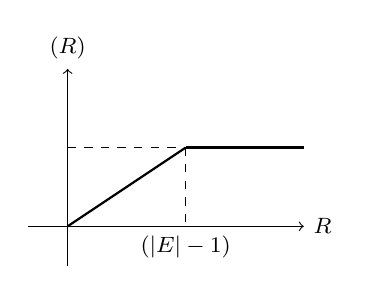
\begin{tikzpicture}
\tikzstyle{every node}=[font= \fontsize{8pt}{10pt}\selectfont]
    \draw [thin,  ->] (0,-0.5) -- (0,2)      % draw y-axis line
        node [above, black] {$\wskc(R)$};              % add label for y-axis
    
    \draw [thin,  ->] (-0.5,0) -- (3,0)      % draw x-axis line
        node [right, black] {$R$};              % add label for x-axis
    
    \draw [draw=black, thick] (0,0) -- (1.5,1);% draw the graph
    \draw [draw=black, thick] (1.5,1) -- (3,1);
    \draw [thin,  dashed] (0,1) -- (1.5,1);
    \draw [thin,  dashed] (1.5,1) -- (1.5,0);
    
    \node [left] at (0,1) {$\wskc$};                % label y-intercept
    \node [below] at (1.5,0) {$(|E|-1)\wskc$};               % label x-intercept
\end{tikzpicture}
% \caption{$\wskc(R)$ curve denoting the wiretap secret key capacity at a given rate $R$ }
% \label{fig:rateregion}
%  \end{figure}
% \begin{theorem}
% Given an irreducible tree-PIN source $\RZ_V$ with a linear wiretapper $\RZ_w$, we have 
% \begin{align*}
% \wskc(R) = \min \left\{\frac{R}{|E|-1}, \wskc\right\} 
% \end{align*}
% where $R$ is the total discussion rate and $\wskc =\min_{e \in E}H(Y_e)$, which is the unconstrained wiretap secret key capacity.
% \end{theorem}
% \begin{proof}
% Since the wiretapper side information can only reduce the secret key rate, $\wskc(R) \leq \skc(R)$. It follows from \cite[Theorem~4.2]{chan19} that $\skc(R) =  \min \left\{\frac{R}{|E|-1}, \skc\right\}$. Therefore, we have $\wskc(R) \leq \min \left\{\frac{R}{|E|-1}, \wskc\right\}$ because $\skc =\wskc$ for an irreducible tree-PIN source with linear wiretapper, which was shown in Theorem~\ref{thm:cwsk:irred}.

% For the achievability part, it is enough to show that the point $((|E|-1)\wskc,\wskc)$ is achievable because the rest of the curve follows from the time sharing argument between $((|E|-1)\wskc,\wskc)$ and $(0,0)$ ---  see Fig.~\ref{fig:rateregion}.

% Let $s:=\wskc=\min_{e \in E}H(Y_e)=\min_{e \in E}n_e$, which is an integer. We will construct our achievable scheme on a sub-source  $\RZ'_V$ of the tree-PIN source $\RZ_V$ by ignoring some edge random variables. More precisely, $\RZ'_V$ is defined on the same tree $T$ with $\RY'_e := \left( \RX_{e,1}, \ldots, \RX_{e,s} \right)$ for each edge $e \in E$, and $\RZ'_i = \left( \RY'_e : i \in \xi (e) \right)$ for $i \in V$. Note that all the edge random vectors $\RY'_e$ have $s$ components. On the other hand, the  wiretapper side information $\RZ_{\opw}$ is the same as that of the original source. 

% Let $\RX' :=(\RX_{e,k}: e\in E, 1 \leq k \leq s)$ and  $\RX'' :=(\RX_{e,k}: e\in E, s < k \leq n_e)$, which is a partition of the underlying components $\RX$ of the original source. This gives rise to a partition of the observations of the wiretapper into two parts: the first part contains observations involving only linear combinations of $\RX'$, and the second part contains linear observations with at least one component from $\RX''$. This means that $\RZ_{\opw}$, after applying some suitable invertible linear transformation, can be written as 
% $$\RZ_{\opw} = \bM \RX' & \RX''\eM \bM \MA & \MB \\ \M0 & \MC \eM ,$$ for some matrices $\MA$, $\MB$, and a full column-rank matrix $\MC$. With $\RZ'_{\opw}=\RX'\MA$ and $\RZ''_{\opw}=\RX'\MB + \RX''\MC$, $\RZ_{\opw} = \bM \RZ'_{\opw} & \RZ''_{\opw} \eM$.

% For a large $n$,  users execute a linear secure omniscience communication scheme $\RF^{(n)}$ on the sub-source $\RZ'^n_V$ with respect to the wiretapper side information $\RZ^n_{\opw}$. Moreover, $\RF^{(n)}$ has the following properties: it achieves perfect omniscience at rate 
% $$\frac{1}{n}H(\RF^{(n)})=H(\RZ'_V)-s=H(\RX')-s,$$ which is the minimum rate of omniscience $\rco(\RZ'_V)$, and it perfectly aligns with $\RZ'^n_{\opw}$, i.e., $H(\RZ'^n_{\opw}|\RF^{(n)})=0$. The existence of such a communication scheme is guaranteed from the proof of Theorem~\ref{thm:cwsk:irred}. After every user recovers the source $\RZ'^n_V$ using $\RF^{(n)}$, they agree on the key $\RK^{(n)}:=\RY'^n_{e_0}$ where $e_0 \in E$ is an edge incident on a leaf node. It is clear that $\RK^{(n)}$ satisfies the key recoverability condition because it is a function of the recovered source $\RZ'^n_V$. It remains to show that $\RK^{(n)}$ satisfies the secrecy condition.

% Since $\RK^{(n)},\RZ'^n_{\opw}$ and $\RF^{(n)}$ are linear functions of $\RX'$, we have  $(\RK^{(n)}, \RF^{(n)}, \RZ'^n_{\opw}) - \RX'^n-\RZ''^n_{\opw}$. Note that $\RZ''^n_{\opw}$ is independent of $\RX'$ because $\MC$ is a full column-rank matrix. As a consequence, $\RZ''^n_{\opw}$ is independent of $(\RK^{(n)}, \RF^{(n)}, \RZ'^n_{\opw})$.  Furthermore, $\RY'^n_{e_0}$ is independent of $\RF^{(n)}$. This can be obtained by combining the perfect omniscience condition, which implies that $H(\RZ'^n_V|\RY'^n_{e_0},\RF^{(n)})=0$ for the leaf node, and the condition on the rate of the communication which is  $H(\RF^{(n)})=H(\RZ'^n_V)-ns=H(\RZ'^n_V)-H(\RY'^n_{e_0})$. Therefore, we have $H(\RY'^n_{e_0}|\RF^{(n)})= H(\RY'^n_{e_0},\RF^{(n)})-H(\RF^{(n)})=H(\RZ'^n_V,\RY'^n_{e_0},\RF^{(n)})-H(\RF^{(n)})=H(\RZ'^n_V)-H(\RF^{(n)})=H(\RY'^n_{e_0})$. The third equality is because $\RY'^n_{e_0}$ and $\RF^{(n)}$ are linear functions of $\RZ'^n_V$. Finally,
% \begin{align*}
%     H(\RK^{(n)}| \RF^{(n)}, \RZ^n_{\opw}) &=  H(\RK^{(n)}| \RF^{(n)}, \RZ'^n_{\opw},\RZ''^n_{\opw})\\
%     &\utag{a}{=}  H(\RK^{(n)}| \RF^{(n)}, \RZ'^n_{\opw})\\
%     &\utag{b}{=} H(\RK^{(n)}| \RF^{(n)})\\
%     &= H(\RY'^n_{e_0}| \RF^{(n)})\\
%     &\utag{c}{=}H(\RY'^n_{e_0})\\
%     &= H(\RK^{(n)})
% \end{align*}
% where (a) follow from the independence of $\RZ''^n_{\opw}$ and $(\RK^{(n)}, \RF^{(n)}, \RZ'^n_{\opw})$, (b) is due that the fact that $\RF^{(n)}$ aligns perfectly with $\RZ'^n_{\opw}$, i.e., $H(\RZ'^n_{\opw}|\RF^{(n)})=0$ and (c) is because $\RY'^n_{e_0}$ is independent of $\RF^{(n)}$.

% Thus we have shown that a secret key of rate $\frac{1}{n}H(\RK^{(n)})=\frac{1}{n}H(\RY'^n_{e_0})=s$ is achievable with a communication of rate $\frac{1}{n}H(\RF^{(n)})=H(\RZ'_V)-s= (|E|-1)s$. So the pair $((|E|-1)\wskc,\wskc)= ((|E|-1)s,s)$  is achievable, which is as desired.
% \end{proof}

% To extend this result to the general tree-PIN case, we will prove the following lemma, which allows us to carry out a reduction to an irreducible source without changing $\wskc(R)$. This lemma along with the above theorem on irreducible sources proves Theorem~\ref{thm:rateconstrained_treepin}. 

% \begin{lemma}\label{lem:irred:rate} 
%  If a tree-PIN source with linear wiretapper $(\RZ_V,\RZ_{\opw})$ is not irreducible then there exists an irreducible source $(\tRZ_V, \tRZ_{\opw})$ such that 
%  \begin{align*}
% &\wskc(\RZ_V\| \RZ_{\opw})(R) = \wskc(\tRZ_V\|\tRZ_{\opw})(R),\\ 
% &H(\RY_e|\op{mcf}(\RY_e,\RZ_{\opw})) = H(\tRY_e),
% \end{align*}
% for all $e \in E$.
% \end{lemma}
% \begin{proof}
% Since $(\RZ_V, \RZ_{\opw})$ is not irreducible, there exists an edge $e \in E$ such that $\RG_e := \op{mcf}(\RY_e, \RZ_{\opw})$ is a non-constant function. Similar to the proof of Lemma~\ref{lem:irred:rate}, we linearly transform $\RY_e$ and $\RZ_{\opw}$ to  $(\RG_e, \tRY_e)$ and $(\RG_e, \tRZ_{\opw} )$, respectively where $ H(\tRY_e)=H(\RY_e|\op{mcf}(\RY_e,\RZ_{\opw}))$. Let us consider a  new tree-PIN  source $\tRZ_V$, which is the same as $\RZ_V$ except that  $\tRY_e$ and $\tilde{n}_e$ are associated to the edge $e$, and the wiretapper side information is  $\tRZ_{\opw}$. Note that $(\tRZ_V, \tRZ_{\opw})$ is also a tree-PIN source with linear wiretapper, and $\RG_e$ is independent of $(\tRZ_V, \tRZ_{\opw})$.

% Since any valid scheme on reduced model $(\tRZ_V, \tRZ_{\opw})$ can be used as a valid scheme on original model $(\RZ_V, \RZ_{\opw})$, we have 
% $$\wskc(\RZ_V\| \RZ_{\opw})(R) \geq \wskc(\tRZ_V\|\tRZ_{\opw})(R).$$

% To prove the reverse inequality, $\wskc(\RZ_V\| \RZ_{\opw})(R) \leq \wskc(\tRZ_V\|\tRZ_{\opw})(R)$, let $(\RF^{(n)},\RK^{(n)})$ be an SKA scheme achieving $\wskc(\RZ_V\| \RZ_{\opw})(R)=:\wskc(R)$. It means that for $\epsilon_n \to 0$ 
% \begin{align*}
%     & \left|\frac{1}{n}H(\RF^{(n)})-R \right|< \epsilon_n ,\quad \left|\frac{1}{n}H(\RK^{(n)})-\wskc(R)\right|< \epsilon_n, \notag\\
%     & I(\RK^{(n)}\wedge\RZ^n_{\opw},\RF^{(n)})< \epsilon_n, \text{ and }
%     \Pr\left[ \exists j\in V \text{ s.t. } \RK_j^{(n)}\neq \RK_1^{(n)}\right]< \epsilon_n. \notag
% \end{align*}
% Note that the condition $I(\RK^{(n)}\wedge\tRZ^n_{\opw},\RG^n_e,\RF^{(n)})=I(\RK^{(n)}\wedge\RZ^n_{\opw},\RF^{(n)})< \epsilon_n$ implies that $I(\RK^{(n)}\wedge\tRZ^n_{\opw},\RF^{(n)}|\RG^n_e)< \epsilon_n$ and $I(\RK^{(n)}\wedge \RG^n_e)< \epsilon_n$, which in turn imply that $H(\RK^{(n)}) -H(\RK^{(n)}|\RG^n_e)< \epsilon_n$ and $\left|\frac{1}{n}H(\RK^{(n)}|\RG^n_e)-\wskc(R)\right|<2\epsilon_n$. The last inequality follows  from the triangle inequality. Since $\frac{1}{n}H(\RF^{(n)}|\RG^n_e)\leq \frac{1}{n}H(\RF^{(n)})$ and  $\frac{1}{n}H(\RF^{(n)}) \to R$, we have  $\limsup \frac{1}{n}H(\RF^{(n)}|\RG^n_e)\leq R$. We just  restrict to the subsequence  whose limit achieves limsup and with an abuse of notation we still index this sequence with $n$. Let $\lim \frac{1}{n}H(\RF^{(n)}|\RG^n_e):=R-\gamma$ for some $\gamma\geq 0$.

% Now we will find  a best realization of $\RG_e^n$ for which the SKA scheme $(\RF^{(n)},\RK^{(n)})$ has desired properties. From all the above conditions, we have 
% \begin{align*}
%     &\left|\frac{1}{n}H(\RF^{(n)}|\RG^n_e)-(R-\gamma) \right| + \left|\frac{1}{n}H(\RK^{(n)}|\RG^n_e)-\wskc(R)\right|+I(\RK^{(n)}\wedge\tRZ^n_{\opw},\RF^{(n)}|\RG^n_e)\\&\mkern 400mu+\Pr\left[ \exists j\in V \text{ s.t. } \RK_j^{(n)}\neq \RK_1^{(n)}\right]< 5\epsilon_n.
% \end{align*}
% We can rewrite it as 
% \begin{align*}
%     &\sum \Pr(\RG^n_e=g^n_e)\left\{\left|\frac{1}{n}H(\RF^{(n)}|\RG^n_e=g^n_e)-(R-\gamma) \right| + \left|\frac{1}{n}H(\RK^{(n)}|\RG^n_e=g^n_e)-\wskc(R)\right|\right.\\&\mkern 100mu\left.+I(\RK^{(n)}\wedge\tRZ^n_{\opw},\RF^{(n)}|\RG^n_e=g^n_e)+\Pr\left[ \exists j\in V \text{ s.t. } \RK_j^{(n)}\neq \RK_1^{(n)}|\RG^n_e=g^n_e\right]\right\}< 5\epsilon_n. 
% \end{align*}
% Since the average is less than $5\epsilon_n$, there exists a realization $\RG^n_e=g^n_e$ such that 
% \begin{align}\label{eq:rate:reduction}
%     &\left|\frac{1}{n}H(\RF^{(n)}|\RG^n_e=g^n_e)-(R-\gamma) \right|\notag +\left|\frac{1}{n}H(\RK^{(n)}|\RG^n_e=g^n_e)-\wskc(R)\right|\notag +I(\RK^{(n)}\wedge\tRZ^n_{\opw},\RF^{(n)}|\RG^n_e=g^n_e)\notag \\&\mkern 400mu+\Pr\left[ \exists j\in V \text{ s.t. } \RK_j^{(n)}\neq \RK_1^{(n)}|\RG^n_e=g^n_e\right]< 5\epsilon_n.
% \end{align}
% Therefore, each term in the summation is less than $5\epsilon_n$. Now we can use the scheme $(\RF^{(n)},\RK^{(n)})$  corresponding to a fixed $\RG^n_e=g^n_e$ on the reduced model $(\tRZ_V, \tRZ_{\opw})$. From \eqref{eq:rate:reduction}, we can say that it is a valid SKA scheme on $(\tRZ_V, \tRZ_{\opw})$  with a key rate of $\wskc(R)$ and a communication rate of  $(R-\gamma)$. Thus,
% \begin{align*}
%     \wskc(\RZ_V\| \RZ_{\opw})(R)= \wskc(R) \leq \wskc(\tRZ_V\|\tRZ_{\opw})(R-\gamma)\leq \wskc(\tRZ_V\|\tRZ_{\opw})(R),
% \end{align*}
% where the first inequality is due the fact that capacity is the maximum of all the achievable rates at a communication rate of $(R-\gamma)$, and the last inequality follows form the  monotonicity of the $\wskc(R)$ curve. This shows that  $\wskc(\RZ_V\| \RZ_{\opw})(R)= \wskc(\tRZ_V\|\tRZ_{\opw})(R)$. Therefore, we can repeat this process until the source becomes irreducible without affecting $\wskc(\RZ_V\| \RZ_{\opw})(R)$.
% \end{proof}

% The result of Theorem~\ref{thm:rateconstrained_treepin} follows by putting the above lemma and theorem together.



 